\chapter{Unsupervised Learning and Clustering}

\section{$k$-means Clustering}

Suppose we have a data set $\MX\in\R^{m \times n}$, where as usual each data point corresponds to $\MX_{i,*}\in\R^n$, and that under reasonable conjecturing or experimentation we determine the data might be separated in groups. One such algorithm would be $k$-means clustering.

First , we need to initialize some parameters. Pick $k$, the number of clusters in which we desire to separate the data points. Choose $M=\{\vmu_1, \vmu_2, \cdots, \vmu_k\} \subset\R^n$ to be arbitrary points in $n$-space. Define $\vpi\in\R^m$ such that $\pi_i = j$ if $\MX_{i,*}$ is the closest to $\vmu_j$. 

The cost function that this learning algorithm will minimize is

$$J(M) = \frac{1}{m} \sum_{i=1}^{m} \norm{ \MX_{i,*} - \vmu_{\pi_i}}_2 $$ 

Finally initialize a counter variable $t=0$, a list $\textit{costs}$ with the initial cost $J(M)$, and a stopping condition $\epsilon>0$. Then, an implementation in pseudo-code, provided below:

\begin{algorithm}
    \caption{$k$-means Clustering}
    \begin{algorithmic}[1]
		\While {True}
		\If {$t>1$ and $|costs[t]-costs[t-1]|<\epsilon$}
		\State break
		\EndIf
		\For {$i$ in range($k$)}
        \State $m_i =\{ \#j \quad st. \quad \pi_j = i$ \}
        \State $\vmu_i = \frac{1}{m_i}\sum_{j:\pi_j=i} \MX_{j,*}$
		\EndFor
		\State Compute new values for $\vpi, J$
		\State $t+=1$
		\State Append $J$ to \textit{costs}
		\EndWhile
	\end{algorithmic} 
\end{algorithm}

Without loss of generality, we will assume that the labels correspond to the first $k$ positive integers (they need not to be, but we can always label them as such.)

First, for each label $i$, we want to consider all the data points that have $i$ as a label with the current vector $\vpi$, and compute the center of those points and set that new point to $\mu_i$.

Doing so for all labels, we will obtain a new $\vmu$, for which we recalculate the vector $\vpi$, and with that a new cost function value $J$.

Then, we repeat this process until the cost function value decreases less than our designated function value (this is determined by the size of the $\epsilon$ constant that we choose at the start.)

\begin{example} 
Consider the following simple case with the following data and $k=3$. 

The data has been marked with red, while the $\vmu$'s have been marked with blue. The black line segments connecting the red points with the blue points represent the values of our vector $\vmu$ (\ref{fig:9.1Ex1}).

Since the data selected exhibits very clear clustering, the algorithm terminates after running a single iteration (\ref{fig:9.1Ex2}).

\begin{figure}[h]
    \centering
    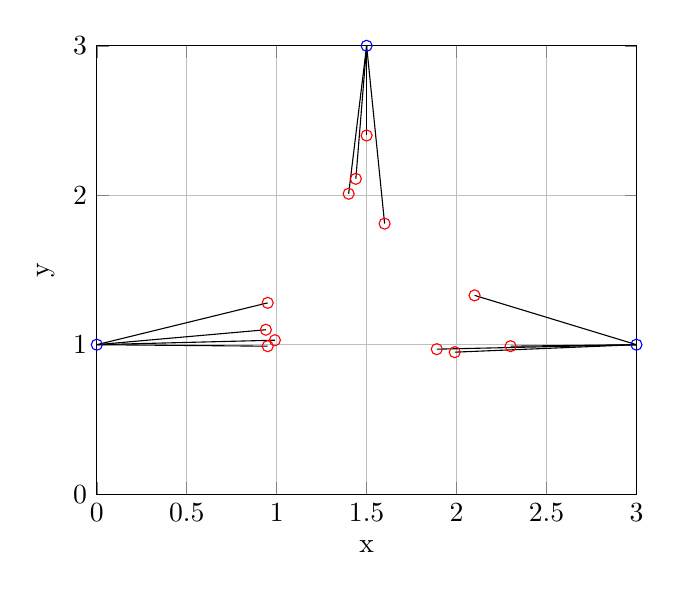
\begin{tikzpicture}
    \begin{axis}
    [
        xlabel={x}, 
        ylabel={y}, 
        grid, 
        xmin=0, 
        xmax=3, 
        ymin=0, 
        ymax=3, 
        tick align=inside
    ]
    \addplot[red, mark=o, only marks] coordinates {
        (0.94, 1.1)
        (0.95, 1.28)
        (0.95, 0.99)
        (0.99, 1.03)
        (1.89, 0.97)
        (1.99, 0.95)
        (2.1, 1.33)
        (2.3, 0.99)        
        (1.5, 2.4)
        (1.4, 2.01)
        (1.44, 2.11)
        (1.6, 1.81)
    };
    \addplot[blue, mark=o, only marks] coordinates {
        (0, 1)
        (1.5, 3)
        (3, 1)
    };
        \addplot[black] coordinates {(0,1) (0.94, 1.1)};
        \addplot[black] coordinates {(0,1) (0.95, 1.28)};
        \addplot[black] coordinates {(0,1) (0.95, 0.99)};
        \addplot[black] coordinates {(0,1) (0.99, 1.03)};
        \addplot[black] coordinates {(3, 1) (1.89, 0.97)};
        \addplot[black] coordinates {(3, 1) (1.99, 0.95)};
        \addplot[black] coordinates {(3, 1) (2.1, 1.33)};
        \addplot[black] coordinates {(3, 1) (2.3, 0.99)};      
        \addplot[black] coordinates {(1.5, 3) (1.5, 2.4)};
        \addplot[black] coordinates {(1.5, 3) (1.4, 2.01)};
        \addplot[black] coordinates {(1.5, 3) (1.44, 2.11)};
        \addplot[black] coordinates {(1.5, 3) (1.6, 1.81)};

    \end{axis}
\end{tikzpicture}
    \caption{Initial $\vmu$ and $\vpi$}
    \label{fig:9.1Ex1}
\end{figure}

\begin{figure}[h]
    \centering
    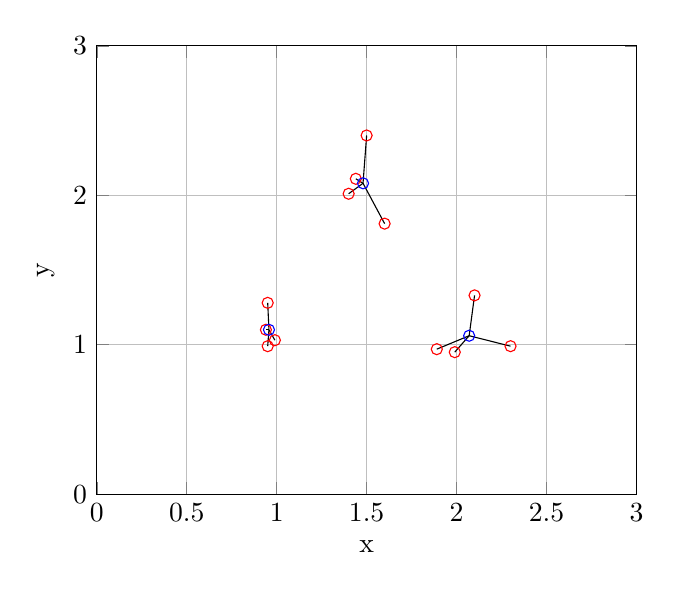
\begin{tikzpicture}
        \begin{axis}
        [
            xlabel={x}, 
            ylabel={y}, 
            grid, 
            xmin=0, 
            xmax=3, 
            ymin=0, 
            ymax=3, 
            tick align=inside
        ]
        \addplot[red, mark=o, only marks] coordinates {
            (0.94, 1.1)
            (0.95, 1.28)
            (0.95, 0.99)
            (0.99, 1.03)
            (1.89, 0.97)
            (1.99, 0.95)
            (2.1, 1.33)
            (2.3, 0.99)        
            (1.5, 2.4)
            (1.4, 2.01)
            (1.44, 2.11)
            (1.6, 1.81)
        };
        \addplot[blue, mark=o, only marks] coordinates {
            (0.957, 1.1)
            (2.07, 1.06)
            (1.48, 2.08)
        };
            \addplot[black] coordinates {(0.957, 1.1) (0.94, 1.1)};
            \addplot[black] coordinates {(0.957, 1.1) (0.95, 1.28)};
            \addplot[black] coordinates {(0.957, 1.1) (0.95, 0.99)};
            \addplot[black] coordinates {(0.957, 1.1) (0.99, 1.03)};
            \addplot[black] coordinates {(2.07, 1.06) (1.89, 0.97)};
            \addplot[black] coordinates {(2.07, 1.06) (1.99, 0.95)};
            \addplot[black] coordinates {(2.07, 1.06) (2.1, 1.33)};
            \addplot[black] coordinates {(2.07, 1.06) (2.3, 0.99)};      
            \addplot[black] coordinates {(1.48, 2.08) (1.5, 2.4)};
            \addplot[black] coordinates {(1.48, 2.08) (1.4, 2.01)};
            \addplot[black] coordinates {(1.48, 2.08) (1.44, 2.11)};
            \addplot[black] coordinates {(1.48, 2.08) (1.6, 1.81)};
    
        \end{axis}
    \end{tikzpicture}
    \caption{$\vmu$ and $\vpi$ after one iteration}
    \label{fig:9.1Ex2}
\end{figure}

\end{example}

\begin{example}
Given a data set of matrices in $\R^{8\times 8}$ representing an $8$-by-$8$ black and white pixel image of handwritten digits, we would like to run $10$-means clustering, in hope that each digit is reasonably clustered (i.e. two digits are close if they are the same, and far apart if they are different.)

Then, after obtaining a value for $\vmu$, we can run predictions on unlabeled data to predict the digit that it corresponds to it with the center closest to it.
\end{example}

\section{Exercises}

\begin{enumerate}
    \item Suppose a streaming service uses cluster analysis to classify users in order to better tailor ads. Explain why this model would struggle to classify a shared account.
    \item Under what circumstances would a non-convex set would not be classifiable with $k$-means clustering?
    \item Although it was suggested that $M$ could be chosen arbitrarily, give an example where a bad initialization of $M$ would lead to the algorithm not producing reasonable clusters.
\end{enumerate}

\section{Solution To Exercises}
\begin{enumerate}
    \item A possible explanation might be that the metrics used are too irregular if there distinct users have sharp differences on their preferences.
    \item Non-convex sets are not captured precisely if distinct groups are too close, since $k$-means clusters data into spheres. However if the sets are far apart from each other, it is possible for the algorithm to classify data properly.
    \item If the set $M$ is initialized with very similar centers, then the algorithm might converge into overlapping spheres.
\end{enumerate}